\documentclass[preprint,amsmath,amssymb,superscriptaddress]{revtex4-1}
\usepackage{graphicx,amsmath}
\usepackage{color}
\begin{document}
\draft


\title{A novel route to the spontaneous formation of porous crystals via viscoelastic phase separation} 

\author{Hideyo Tsurusawa} 
\affiliation{Institute of Industrial Science, University of Tokyo, 4-6-1 Komaba, Meguro-ku, Tokyo 153-8505, Japan}
\author{John Russo}
\affiliation{Institute of Industrial Science, University of Tokyo, 4-6-1 Komaba, Meguro-ku, Tokyo 153-8505, Japan}
\affiliation{ {School of Mathematics, University of Bristol, Bristol BS8 1TW, United Kingdom} }
\author{Mathieu Leocmach}
\affiliation{Institut Lumière Matière, CNRS UMR 5306, Université Claude Bernard Lyon 1, Université de Lyon, Lyon, 69622 Villeurbanne Cedex, France}
\author{Hajime Tanaka  \footnote{e-mail: tanaka@iis.u-tokyo.ac.jp}}
\affiliation{Institute of Industrial Science, University of Tokyo, 4-6-1 Komaba, Meguro-ku, Tokyo 153-8505, Japan}

\date{Received \today}

\begin{abstract}
{\bf
Viscoelastic phase separation of colloidal suspensions can be interrupted to form gels either by 
%the glass transition, with the formation of colloidal gels~\cite{poon2002,zaccarelli2007,piazza1994phase,verhaegh1997transient,tanaka1999colloid,lu2008gelation}, or by crystallization, which results in the formation of a crystalline network~\cite{soga1999metastable,fortini2008crystallization,perez2011pathways,sabin2012}. 
glass transition~\cite{poon2002,zaccarelli2007,piazza1994phase,verhaegh1997transient,tanaka1999colloid,lu2008gelation} or by crystallization~\cite{soga1999metastable,fortini2008crystallization,perez2011pathways,sabin2012}. 
%But while the former process has been studied in detail, the latter has never been observed experimentally at a single-particle level and it is thus lacking a microscopic understanding. 
With a new confocal microscopy protocol, we unveil a novel crystallization pathway to sponge-like porous structures in a colloid-polymer mixture undergoing viscoelastic gas-liquid phase separation. We show that crystallization leads to a network structure different from the original phase separation pattern. Crystals nucleate inside the liquid network, but grow past it by direct condensation of the gas phase on their surface, i.e. desublimation, driving evaporation of nearby liquid. %The latter processes via the gas phase has been overlooked so far. %This process represents the colloidal analogue of the Bergeron process~\cite{glickman2000glossary}, which explains the formation of ice crystals in mixed phase clouds and is at the origin of rain. Our finding gives us full experimental access to the kinetic pathway of this poorly understood phenomenon important for climate science. 
%The key is complex dynamic interplay involving the three phases upon simultaneous occurrence of two non-equilibrium phenomena, phase separation and crystallization. 
We argue that similar crystal-gel states can be formed as the result of the gas-liquid phase separation of any crystallizable components, such as monoatomic and molecular systems, if dynamics of the liquid phase is slow enough to induce viscoelastic phase separation, but fast enough to prevent immediate vitrification. This mechanism will provide a novel single-step pathway to form nano-porous crystals of metals and semiconductors without dealloying \cite{erlebacher2001evolution}, which may be important for catalytic, optical, sensing, and filtration applications \cite{ding2004nanoporous,ding2009nanoporous, wittstock2010nanoporous}.
%, but also sheds new light on crystal network formation in more complex systems such as magma \cite{philpotts1998role}, biominerals \cite{rousseau2005multiscale}, and foods \cite{deman1987fat}.}
}
\end{abstract}


\maketitle

Crystallization plays a fundamental role in many processes occurring in nature, such as cloud composition, and in technological applications
that are at the core of the chemical, pharmaceutical, and food industries.
Many of the properties of crystals, like the shape, spatial arrangement, polymorph type, and size distribution of the crystallites, depend on the conditions at which
the nucleation process took place. Controlling the early stages of crystallization is thus of fundamental importance in order to
obtain in a reproducible manner crystals with the desired properties. 

Under usual conditions, the nucleation stage involves a very small number of molecules, of the order of 10-1000 molecules.
This has severely limited the possibility to observe the nucleation process directly, and has also posed limits on
models based on macroscopic thermodynamic properties. 
The inability to directly observe the nucleation process is also a limit to our understanding of its kinetic pathway. 
Classical Nucleation Theory assumes the crystallization processes to occur in one step,
where the transition can be described by just one reaction coordinate. An example is the formation of an ordered crystalline nucleus
directly from the supersaturated solution. But the possibility of different pathways has recently come to prominence with
the discovery of two-step nucleation pathways, where crystallization is proceeded by the formation of dense liquid  droplets as an intermediate step~\cite{ten1997enhancement,SearR,savage2009experimental,vekilov2010two,palberg2014crystallization}.
Understanding the process of crystal formation in mixed-phase systems (composed of gas, liquid, and solid phases) is thus
of great importance for a variety of systems, from protein solutions to clouds. 

Colloidal suspensions offer a system where the crystallization process in a mixed-phase environment can be observed with single-particle
resolution, and at the same time scales over which nucleation takes place. In colloids with short-range attractions the liquid-gas transition 
becomes metastable with respect to crystallization~\cite{anderson2002insights,lekkerkerker2011colloids}, and can form gels
by viscoelastic phase separation \cite{tanaka1999colloid,tanaka2000viscoelastic}, with the coexistence of a dense liquid phase with slow dynamics and a dilute gas phase with fast dynamics. 
This difference in the viscoelastic properties between the two phases allows the system to form a space-spanning 
network structure of the liquid phase, even if it is the minority phase. The network is fractal and its dynamic structure factor shows a stretched-exponential decay to a finite
plateau~\cite{krall1998internal,solomon2001dynamic,romer2000sol}. 
During phase separation, the density of the liquid phase increases towards the glass-transition density, leading to slow glassy dynamics.
At the glass transition point, the percolated network structure is dynamically stabilised by vitrification 
of the dense liquid phase~\cite{pusey1993dynamics,piazza1994phase,ilett1995phase,verhaegh1997transient,tanaka1999colloid,foffi2002,buzzaccaro2007sticky,zaccarelli2007,lu2008gelation,zaccarelli2008gelation,testard2011}.  
More precisely, the dynamical stabilization is due to percolation of locally favoured structures, which are locally stable non-crystalline structures \cite{royall2008g}.

% Gels and glasses are two important non-ergodic disordered states, which are very important 
% in our life and nature~\cite{anderson2002insights,lekkerkerker2011colloids}.
% The dynamical arrest of colloidal gels and glasses is believed to originate from a dynamical transition to the same non-ergodic disordered glass state, i.e., vitrification. The only difference comes from the fact that the former is formed by densification induced by phase separation and thus is spatially heterogeneous, whereas the latter is formed by uniform densification and is thus spatially homogeneous.
% Gels are distinct from glasses because of their heterogeneous network structure, which gives them properties intermediate between
% those of a solid and a fluid phase, and allows the coexistence of two properties usually incompatible with each other, 
% elasticity and fluidity. 
% The elasticity of gels originates from the percolated network structure and the resulting space-spanning connectivity. 
% At the same time a fluid component can easily flow through the elastic network.
% There are two types of gels with such characteristics: one is a network structure stabilized by stable crosslinks, and the other is a phase-separated structure frozen by dynamical arrest due to vitrification.
% Many chemical and physical gels belong to the former category, in which the size of network pores is rather small and 
% the fluid transport is not so efficient. On the other hand, gels made of spherical colloids and proteins 
% with attractive interactions belong to the latter category. 
% This type of gels are formed by viscoelastic phase separation \cite{tanaka1999colloid,tanaka2000viscoelastic} into a dense liquid phase with slow dynamics and a dilute gas phase 
% with fast dynamics. This difference in the viscoelastic properties between the two phases allows the system to form a space-spanning 
% network structure of the liquid phase, even if it is the minority phase. The network is fractal and its dynamic structure factor shows a stretched-exponential decay to a finite
% plateau~\cite{krall1998internal,solomon2001dynamic,romer2000sol}. During phase separation, the density of the liquid phase 
% increases towards the glass-transition density, leading to slow glassy dynamics.
% At the glass transition point, the percolated network structure is dynamically stabilised by vitrification 
% of the dense liquid phase~\cite{pusey1993dynamics,ilett1995phase,verhaegh1997transient,tanaka1999colloid,foffi2002,buzzaccaro2007sticky,zaccarelli2007,lu2008gelation,zaccarelli2008gelation,testard2011}.  
% More precisely, the dynamical stabilization is due to percolation of locally favored structures, which are locally stable non-crystalline structures \cite{royall2008g}.
% Since ``glass'' is the term used for bulk, this may be a more appropriate way to express the mechanism of dynamical arrest. 
% This type of gels are made by phase separation. Thus, the structure is intrinsically heterogeneous, and the network pore size is usually 
% much larger than gels made of stable crosslinks, resulting in a high fluid transport ability. 

Unlike the above standard scenario of colloidal gelation, it is known that phase separation can also be arrested by crystallization, if the process takes place below the melting point of a component of a mixture~\cite{tanaka1985new}. Indeed the possibility of a different class of gels, which are stabilized by crystallization, 
was suggested by numerical simulations~\cite{soga1999metastable,fortini2008crystallization,perez2011pathways} and observed in microgravity experiments \cite{sabin2012}. 
For colloidal systems, we can in principle access structural evolution in real time at a single-particle level; however, there has so far been no confocal microscopy  
study on the dynamical process of crystal-gel formation. 
For confocal microscopy experiments on colloid gelation, colloid-polymer mixtures have so far been used as a model system. 
The main difficulty consists in the preparation protocol of such a colloid-polymer mixture, where before observation of its dynamics shaking or applying shear is necessary to prepare an initial homogeneous state. This introduces turbulent flows at the beginning of the process, and also does not allow the
observation of the initial stages of crystallization. This initial perturbation may even alter the selection of the final non-equilibrium arrested state.  
In our experiments we instead succeed in building a novel protocol that allows the time evolution of the system to be observed directly
under the confocal microscope from the very early stages and in a quiescent situation without introducing fluid flows. 

In this Letter, we show that, for low polymer concentration, the system can undergo a novel crystallization pathway that leads to the formation
of crystalline droplets. These droplets originate from crystal seeds that form inside the liquid branches of the spinodal aggregate of network morphology, and then grow by direct condensation from the gas phase. The process is analogous to the Bergeron process of ice formation in mixed phase clouds, where ice droplets grow at the
expense of the supercooled liquid droplets due to their lower saturated vapour pressure. 
This is speculated to be the primary mechanism for the formation of raindrops. 
Differently from the standard crystal-gel scenario, where crystals only nucleate and grow inside the dense branches of the gel, becoming dynamically arrested, we show that the kinetic
pathways involving the gas phase (predominanlty the Bergeron process, but also Ostwald ripening) play a fundamental role. We also observe that increasing the strength of the interparticle attraction
(by increasing the polymer concentration), instead of forming crystal gels, the system undergoes the classical gelation process, in which
phase separation is interrupted by vitrification~\cite{verhaegh1997transient,tanaka1999colloid,Royall2007,lu2008gelation}. 


In our experimental setup, the sample cell is put in contact with a reservoir of a salt solution through a semi-permeable membrane (see Methods 
on the details of our experiments).
At $t=0$, the increase in the concentration of salt ions within a few Brownian times ($\tau_B$) screens the Coulombic repulsion between colloidal particles,
which are then subject to attractive depletion forces, making the system thermodynamically unstable and leading to phase separation. 
%In the following we discuss all the stages of the formation of the crystal gels: phase separation, stress-driven agein and crystallization.
The experimental data are taken at two different volume fractions ($\phi\approx 0.13$ and $\phi\approx 0.30$) and for different values
of the polymer concentration, $c_p=0.38,0.48,0.57,1.07$ mg/g for $\phi\approx 0.30$ and $c_p=0.82,1.36$ mg/g for $\phi\approx 0.13$.
In Fig.~\ref{fig:phase_separation}a, we superimpose the state points with the phase diagram, which we calculated from generalised free volume theory~\cite{Fleer2008} using the experimental values for the size of the colloids, the radius of gyration of the polymer, and the polymer concentration (see Methods).
For each state point, scans were made at early times (every $10$~s, i.e. $4\tau_B$) and at the late stage (every $30$~s) of the gelation process. 


%
%\subsection*{Phase separation}
%
%In Fig.~\ref{fig:gel}a we show the cluster size distribution for all state points at their gelation point. The decay of the distribution
%follows different power laws $n(s)\sim s^\tau$, where $\tau$ is the Fisher exponent \cite{family2012kinetics}.
%For state points with $\phi\approx 0.30$ the decay is well described by the three dimensional (3D) random percolation exponent $\tau=2.18$ \cite{family2012kinetics}.
%For state points with $\phi\approx 0.13$, on the other hand, the decay appears to be slower, close to the diffusion limited cluster aggregation (DLCA) 
%exponent $\tau=1.8$ \cite{family2012kinetics}. While it is plausible that gelation at lower volume fraction occurs through cluster aggregation, especially given 
%the high polymer concentration of these state points, we have to warn that the cluster size distribution is very sensitive to
%experimental conditions and statistical noise (which is high in our case since the distributions are extracted from a single frame).
%Other measures of fractal dimensions (see below) will in fact suggest that also the $\phi\approx 0.13$ states belong to the random gel universality class.
%
%Next we show in Fig.~\ref{fig:gel}b the radius of gyration $R_{\rm g}$ for the clusters of size $s$ at the gel point. All clusters, irrespective
% of the state point, follow the power-law: $R_{\rm g}\sim s^{2/D}$, with $D=2.53$ the fractal dimension in the random gelation
% universality class \cite{family2012kinetics}. So far, we have thus proven that, in the initial stages of phase separation, the liquid branch is
% formed by colloidal particles that aggregate to form a random gel.
% 
% Even after a gel is formed, the system keeps evolving.
% However, since a gel has an elasticity due to its space-spanning connectivity, the process should be markedly different from 
% ordinary fluid phase separation. Now we consider this unique feature of the coarsening of a gel network.  
% 
% \subsection*{Stress-driven ageing}
% 



As described above and also in Methods, salt injection initiates liquid-gas phase separation of the colloidal suspension. 
All samples share the same early stages of spinodal decomposition. 
A typical phase ordering process observed at $\phi\approx 0.30$ and $c_p=0.38$ mg/g can be seen in Supplementary Movies 1 and 2. 
Due to strong dynamical asymmetry between colloids and the solvent \cite{tanaka1999colloid}, the colloidal particles start aggregating, 
eventually forming a percolating network. Thus, a dense network (liquid) coexists with freely diffusing monomers (gas).
In Fig.~\ref{fig:phase_separation}a, the state points which did not phase separate are indicated with open triangles, while
the other symbols indicate samples undergoing phase separation. The (black) continuous line is the gas spinodal computed from free volume theory,
and it is in good agreement with our experimental points (the small discrepancy at small colloidal volume fractions 
is common in free volume theory)~\cite{Royall2007,lu2008gelation}. 
The topology of the network is similar to all our samples at the initial stages. 
This is shown for example in Fig.~\ref{fig:phase_separation}b, where we plot the radius of gyration of colloidal clusters ($R_g$)
as a function of the cluster size ($s$) at the percolation point. Two particles belong to the same cluster if their distance is
within the first peak of the radial distribution function. All samples show the same scaling law, $R^2_{\rm g}\sim s^{2/D}$, which is compatible with
the random gelation universality class exponent ($D=2.53$) as shown by the dashed line in Fig.~\ref{fig:phase_separation}b
(we do not imply that the formation of the network follows the random gelation universality class, just that our
fractal dimension is compatible with it).

%%%%
%Previous simulation results~\cite{tanaka2000,tanaka2007spontaneous,furukawa2010key} have suggested that hydrodynamic interactions play a key role in the process of colloidal gelation. Without hydrodynamic interactions, particles have the tendency to aggregate in compact structures and subsequently form thick network structures. This also limits the possibility to form arrested gel states only at relatively high volume fractions. With hydrodynamic interactions, particles first form a transient gel even at very low volume fractions, and only later they increase the number of nearest neighbours to minimize the energy of the structure. Thus, hydrodynamic interactions lead to the formation of gels that are very far from equilibrium and under a strong thermodynamic driving force towards more stable compact structures. The resulting transition from open to more compact networks occurs only through the breaking of the bonds that have accumulated more stress. The process was called stress-driven ageing~\cite{
%tanaka2007spontaneous}, which is characteristic of viscoelastic phase separation \cite{tanaka2000viscoelastic}. Below we provide the first experimental proof of this process.
 
%In Fig.~\ref{fig:stress}a, we plot the fraction of liquid and gas particles as a function of time during phase separation at the state points of $\phi\approx 0.13$. We observe that at high polymer concentration ($c_p=1.36$, dashed lines) both the liquid and gas branch change monotonically with time as the phase separation proceeds. At low polymer concentration ($c_p=0.82$, continuous lines), on the other hand, we find a non-monotonic evolution of both the liquid and gas branches, which is signalling a structural reorganization of the network. To prove that this is indeed a stress-driven ageing process, in Fig.~\ref{fig:stress}b we plot the average number of bond-breaking events for the low-polymer concentration state point. The figure clearly shows that the network restructuring follows a peak in the number of bond-breaking events. We have thus found direct evidence of the stress-driven ageing process in colloidal gels that is a direct consequence of the formation of a thin network with the help of 
hydrodynamic interactions in the first stages of the aggregation process.
 
%In Fig.~\ref{fig:stress}c we plot the time evolution of the structure factor, $S(q)$, for the state point undergoing network reorganization $\phi\approx 0.13$ and $c_p=0.82$. The time of network reorganization as found in Fig.~\ref{fig:stress}a and b corresponds to a steep increase of the low wavenumber scattering from the network, that signals the coarsening of the network structure. 

%The same conclusions also hold for the state point at $\phi\approx 0.30$. We observe network restructuring only for the state point at lower polymer concentration, $c_p=0.38$. Interestingly, this is also the only state point that undergoes crystallization, meaning that the coarsening of the network of the dense liquid phase and the resulting formation of a wider liquid branch is a necessary condition for crystallization. 

%%%

While sharing similar structural properties at early times, the samples show significantly different behaviours in the later stages of the phase separation process.
To examine this in more detail, we plot in Fig.~\ref{fig:phase_separation}c the structure factor for the final stages of the gelation process for all state points.
Calculation of the structure factor is done with the Hanning window function, to minimize boundary effects.
The figure shows that at low wavenumber $q$, the structure factor displays fractal scaling compatible with Guinier law, $S(q)\sim q^{-D}$.
But a difference in the fractal dimension $D$ between the $\phi\approx 0.30$ and $c_p=0.38$ mg/g state point and other state points starts to become visible. In fact, while states
with high polymer concentration retain the exponent $D=2.5(3)$, 
which is the random gel universality class exponent, as we also observed in the early stages of the gelation process (see Fig.~\ref{fig:phase_separation}b),
the state point with low polymer concentration ($\phi\approx 0.30$ and $c_p=0.38$ mg/g) displays the biggest deviation from that exponent. In the figure we also
plot the exponent $D=3$, which corresponds to volume growth, which we will show in the following analysis to be the correct exponent for this state. 
The difference is due to the onset of crystallization in the low-polymer concentration sample. This is already evident in the high $q$ behaviour of
the structure factors (Fig.~\ref{fig:phase_separation}c), where the diffraction planes appear as sharper peaks for $\phi\approx 0.30$ and $c_p=0.38$ mg/g.

To gain additional insight, in Fig.~\ref{fig:phase_separation}d we plot the average local volume fraction as a function of the number of neighbours.
\textcolor{red}{The volume fraction is obtained by computing the Voronoi diagram of each configuration,
which uniquely assigns a volume to each colloidal particle.}
For all state points, we can see that the average volume fraction of a colloidal
particle increases with its number of neighbours. Approaching close packing (12 neighbours), we clearly see two families of curves. The state point
at $\phi\approx 0.30$ and $c_p=0.38$ mg/g reaches close packing at a volume fraction of around $\sim 68\%$, which is in reasonable agreement with the
volume fraction of the stable crystal phase~\cite{ilett1995phase}. All other state points, instead, reach close packing at a volume fraction $\sim 64\%$, which is
indeed close to the volume fraction of the attractive glass state~\cite{pham2002multiple}. 
%(\textbf{the absolute values of these volume fraction are not totally convincing, probably because of a not optimal estimate of the size of the colloids. We should run the code of Mathieau with size detection}). 
This result clearly indicates that the state point at $\phi\approx 0.30$ and $c_p=0.38$ mg/g follows a different arrest mechanism, in which phase separation
is arrested by crystallization and not by glassiness. Although our estimation of the absolute volume fraction may involves systematic errors of a few \%, the trend should be robust~\cite{Poon2012}.


% 
%  REINTREGRARE
% while the crystallizing state point shows a scaling compatible with $D=3$, which
% signals compact crystalline nuclei. At high $q$, the first signals from diffraction planes are also evident in the $\phi\approx 0.30$ and $c_p=0.38$ state
% point. This suggests that the space filling network is composed of crystalline aggregates, differently from the fractal branches which characterize the
% spinodal liquid. Also this suggests that the growth mechanism of the crystal is not simply due to filling of the spinodal liquid network, as was
% instead observed in Ref.~\cite{soga1999metastable,fortini2008crystallization,perez2011pathways} for brownian dynamics simulations.

% 
% 
% \begin{figure}
%  \centering
%  \framebox{Phase diagram\hfill}
%  \includegraphics[width=8cm]{oldfig/fig3b}
%  \includegraphics[width=8cm]{oldfig/fig3c}
%  % crystal_size.eps: 0x0 pixel, 300dpi, 0.00x0.00 cm, bb=(atend)
%  \caption{{\bf Two types of arrest mechanism leading to gel formation.} \textbf{a,} Phase diagram \textbf{b,} Local volume fraction around a colloidal particle, as a function of the number of nearest neighbours of the particle.
%  Different lines represent the different state points. {\bf c,} Structure factors for the late stages of the gelation process.} 
%  \label{fig:statepoints}
% \end{figure}

A direct analysis of the colloidal positions at long times confirms that indeed the new structure obtained at
$\phi\approx 0.30$ and $c_p=0.38$ mg/g has different morphological properties than usual colloidal gels.
We directly compare the two structures in Fig.~\ref{fig:network}, where Gaussian filtering is used to depict the network structure as a continuous field.
Panel a presents the results for high
polymer concentration gel, $c_p=1.07$ mg/g; panel b presents the results for the low polymer concentration sample, $c_p=0.38$ mg/g.
The comparison shows that the new arrest mechanism produces a network structure with bigger pores, smoother surfaces, and thicker strands (panel b) compared
to the colloidal gel sample (panel a). The bottom row shows the individual particle positions for slabs with a thickness of 5 particle diameters.
From the figure it is immediately clear that the network strands at low polymer concentration are crystalline. The new arrest mechanism thus
involve the formation of a crystal-gel network. In order to explain the morphological differences between colloidal gels and crystal-gels,
we now consider the kinetics of formation in our samples. 


To confirm the formation of crystalline seeds, we adopt bond orientational analysis to detect which particles are in crystalline environments~\cite{russo2013interplay}. 
With this analysis we reveal that crystallization events indeed start occurring for the state point $\phi\approx 0.30$ and $c_p=0.38$ mg/g, which has the lowest
polymer concentration of all state points. This is shown in Fig.~\ref{fig:crystals}a, where the black line indicates the average size of the crystallites, 
while the red line indicates the average number of crystallites as a function of time. The number of crystallites first rapidly increases as nucleation events
start occurring inside the liquid network, but eventually starts decreasing as the different crystallites grow and merge with each other.
%The average size of the crystals shows an interesting linear growth regime for $100<t<600$. This linear growth regime goes past the time
%of coalescence of nuclei, so a first speculation is that it could be due to the compensation of the following two effects:
%\begin{itemize}
% \item diffusive growth of the nuclei, which scales like $t^{1/2}$
% \item coalescence growth, which should scale faster than $t$, maybe $t^2?$
%\end{itemize}
All other state points show only negligible signs of crystallization. In particular, for state points with $\phi\approx 0.30$, increasing
polymer concentration drastically reduces the amount of crystals. This is in agreement with the
idea of enhanced crystallization rates near metastable critical points~\cite{ten1997enhancement,olmsted1998spinodal} and the
results of Refs.~\cite{soga1999metastable,fortini2008crystallization,perez2011pathways},
which speculated two different arrest mechanisms: crystallization at low polymer concentration, and dynamic arrest at high polymer concentrations.

While nucleation always occurs inside the liquid branches of the phase-separating network, we suggest here the presence of a new growth channel
which was neither considered nor observed before. In the following we will show that the growth mechanism of the crystal is not only due to filling of the spinodal liquid network, as was observed in Refs.~\cite{soga1999metastable,fortini2008crystallization,perez2011pathways} for Brownian Dynamics simulations, but also involves 
evaporation of the liquid phase and subsequent direct condensation of the gas phase on the crystalline seeds. 
To confirm the presence of the two processes, we plot in Fig.~\ref{fig:crystals}b the gyration radius of individual crystalline nuclei for the state point 
$\phi\approx 0.30$ and $c_p=0.38$ mg/g. The results show that the crystal growth follows two different scaling laws: at small crystalline sizes it scales with 
a fractal dimension close to random percolation ($D=2.53$), while at large sizes it scales as $D=3$, as in compact crystal growth. This demonstrates that, while 
small crystalline nuclei are nucleated inside the phase-separated liquid branches, once they reach the transverse size of the liquid branch, the growth 
follows a volume growth with the formation of isotropic crystal droplets. The same scaling law was suggested in the analysis of the
structure factors, Fig.~\ref{fig:phase_separation}c, but here it is shown directly by the analysis of the gyration radius. 

\textcolor{red}{Next we analyse in detail the crystallization trajectory, distinguishing between the different process responsible for the
crystallization of the phase separated network.
Supplementary Movie 2 shows the confocal microscopy video for the crystallizing sample at $\phi\approx 0.30$ and $c_p=0.38$ mg/g,
where the process of crystal growth by direct attachment of gas particles can be observed directly. 
From the trajectory, we extract slabs of 10 particle diameter thickness for configurations at different times, shown in Fig.~\ref{fig:transitions}a. 
Particles are coloured according to their phases (gas, liquid, and crystal). For the classification criteria see the \emph{Methods} section. The figure shows the first nucleation 
events inside the liquid network (left panel). At the same time liquid regions that have not crystallized start evaporating, and the gas phase contributes to the growth of nuclei (middle panel). Finally the different nuclei coalesce (right panel). Note that the network pattern changes between $t=2055\,\tau_B$ (left panel) and $t=5577,\tau_B$ (middle panel): not all liquid
branches of the network crystallize due to evaporation. The crystal-gel structure instead persists, as seen by comparing $t=5577,\tau_B$ (middle panel) and $t=12098,\tau_B$ (right panel).}

\textcolor{red}{
Next we show in Fig.~\ref{fig:transitions}b the fraction of particles in each different phase for the crystallization trajectory at
$\phi\approx 0.30$ and $c_p=0.38$ mg/g, after the liquid-gas phase separation has occurred.
For the classification criteria see \emph{Methods}.
The process of crystallization is characterized 
by a steep decrease in liquid particles, as they transform into small crystalline nuclei inside the liquid domains. This decrease
is then accompanied by an increase in the fraction of gas particles: as the first crystals start to reach the gas phase, liquid particles evaporate 
to the gas phase due to the higher vapour pressure of the liquid phase compared to the crystalline phase. After the onset 
of a steady-state gas population, there are three growth channels for the crystal. Direct crystallization is the process by which 
crystals grow by incorporating nearby liquid particles. In the Bergeron process, liquid droplets first evaporate and the resulting gas phase 
contributes to the growth of crystalline regions. Ostwald ripening is instead the process by which small crystallites sublimate, and colloidal
particles are transferred to larger nuclei. In order to assess the relative importance of these three growth channels, we analyse the trajectory, and, for every time frame, assign each particle a state between gas, liquid and crystal. In order to minimize short-term fluctuations, the state of each colloidal particle is time averaged for $50\,\tau_B$. We then measure the fraction of trajectories with different transition histories.
Direct crystallization accounts for 54\% of particles trajectories in which
gas or liquid particles transition to the crystal state without liquid evaporation or crystal de-sublimation. The Bergeron process accounts for 35\% of particle trajectories in which liquid particles
transition to the gas state before crystallizing. Ostwald ripening accounts for 11\% of particle trajectories in which crystal particles transition to the gas state before returning
to the crystal state. The different crystallization channels are depicted in the diagram of Fig.~\ref{fig:transitions}c.}

\textcolor{red}{
In Supplementary Information we confirm these results with a detailed analysis of transition probabilities, including a state for surface particles that are in contact.
to crystalline particles.
While the direct freezing of the fluid represents the major contribution to the nuclei growth, the kinetic path via the gas phase (gas$\rightarrow$crystal), also plays a crucial role,
especially in determining the morphology of the porous crystal, as we discussed above. In this context the Bergeron process~\cite{glickman2000glossary,morrison2012resilience}
plays a considerably more important role than Ostwald ripening.}

% 
% Here we mention the simulations closer to our experimental results~\cite{fortini2008crystallization}.
% It was shown there that close to the metastable liquid-gas critical point, the gelation process is arrested by
% crystallization, while at higher polymer concentration by slow dynamics. This is roughly what we observe in
% our experiments, but there is a crucial difference. In the simulation results~\cite{fortini2008crystallization} the kinetic
% pathway at volume fraction $\phi\approx 0.30$ consists of the following three steps: 
% spinodal decomposition; nucleation of crystalline nuclei within the fluid branches;
% growth of crystalline clusters until the whole spinodal structure is crystalline.
% As shown above, the last step appears to be markedly different in our experiments.
% More precisely, at $\phi\approx 0.30$ and polymer concentration $c_p=0.38$ we also observe the first two steps, 
% but the growth process is entirely different. Instead of growing inside
% the spinodal aggregate, the small nuclei grow by adding colloids directly from the gas phase. 

%\subsection*{Discussion and conclusions}
The first stages of gelation always involve spinodal decomposition with the formation
of liquid network by viscoelastic gas-liquid phase separation. 
% Due to hydrodynamic interaction, the network is locally stretched, and the accumulation of mechanical stress on some bonds causes some
% of them to break and the network to reorganize in a more compact and larger structure. This occurs only at low polymer concentration,
% while at high polymer concentrations the bonds are too strong to break. This will eventually dictate which arrest mechanism
% is available to the system.
Depending on the polymer concentration, there are two possible arrest mechanisms. 
(a) Crystallization, observed at $\phi\approx 0.30$ and $c_p=0.38$ mg/g, small crystalline nuclei appear inside the liquid network, reach the surface 
 of the liquid branches, and then grow by addition of particles from the gas phase. The final structure is a network of crystal droplets,
 as confirmed by the fractal dimension of the branches, the volume fraction of the particles within the branches, and bond orientational analysis. 
(b) Dynamic arrest, particle arrest when the dynamics inside the liquid branch becomes slow, which should happen at the intersection of the
 glass line with the liquid side of the coexistence curve. 


The Bergeron process is also the primary mechanism for the formation of rain drops in clouds~\cite{glickman2000glossary,morrison2012resilience}.
In clouds there is a mixture of ice crystals and supercooled water. The vapour phase is in coexistence with the liquid phase, but is supersaturated
with respect to the ice crystals. This causes the water droplets to evaporate and sublimate directly on the ice crystals. Our system can then
be regarded as a colloidal analogue for this important process, which, for the first time, we can observe at the single-particle level.  

The process of formation of ``crystal gels'' may be generic to many other 
systems. The requirements are (i) the presence of gas-liquid phase separation below the melting point of a crystal, (ii) 
weak or little frustration against crystallization (in our case, the use of monodisperse colloids), 
(iii) dynamical slowing down in a supercooled liquid state, which is necessary to induce viscoelastic phase separation leading to the formation 
of a network structure of the minority liquid phase, and (iv) the degree of supercooling is low enough to avoid a high rate of densification of the liquid phase 
leading to vitrification.   
Many monoatomic and single-component molecular systems can satisfy all these conditions in a certain range of the temperature and pressure. 
This can be seen, for example, by looking at the phase diagram of a Lennard-Jones liquid \cite{lodge1997brownian}, which represents many molecular systems 
without specific directional interactions. 

Usually, monoatomic systems are very poor glass-formers and thus have not been expected to form gels. 
However, our mechanism provides a novel kinetic pathway to spontaneously form network or porous structures made of crystals.  The fact that crystals outgrow from the liquid network means that well-ordered crystal planes appear on the surface of the porous structure (see Fig. 2b), which is crucial for catalytic and sensing applications. So we believe that crystal gels are an important class of heterogeneous non-ergodic states in nature 
and industrial applications, although they have not attracted much attention so far.  
For example, nano-porous crystals of noble metals such as Au have special functions associated with ultra-high interfacial area and connectivity of pores, which are relevant to catalytic, optical, sensing, super-capacitor, and filtration applications 
\cite{ding2004nanoporous, ding2009nanoporous, wittstock2010nanoporous,fujita2012atomic}. Usually such nano-porous materials are formed via at least two steps: for example, phase separation and dealloying of a mixture
\cite{erlebacher2001evolution}. Unlike such a method, our novel mechanism allows us to spontaneously form sponge-like nano-porous crystals \emph{in a single step}, 
which may have an impact on many applications. 
We note that laser ablation of metals is a promising method for this purpose \cite{povarnitsyn2013mechanisms}.
We also speculate that our scenario could play a role in the formation of crystal networks observed in dynamically asymmetric mixtures, 
which includes magma \cite{philpotts1998role}, biominerals \cite{rousseau2005multiscale}, and foods \cite{deman1987fat}. 

\vspace{1cm}
\noindent
{\bf METHODS}

\noindent
{\bf Experiments}

We use \textsc{pmma} (poly(methyl methacrylate)) colloids sterically stabilized with methacryloxypropyl terminated \textsc{pdms}(poly(dimethyl siloxane)) and fluorescently labelled with rhodamine isothiocyanate chemically bonded to the \textsc{pmma}. 
The average colloid diameter is 2.2 $\mu$m, measured via the diffusion constant in dilute conditions without polymer. The Brownian time is $\tau_B \approx 2.3$ s. 
We assess that the size distribution of our particle is Gaussian with a polydispersity below 5\% via direct confocal measurements~\cite{Leocmach2013}.
This small polydispersity allows crystallization.
We disperse the particles in refractive index and density matching mixture of cis-decalin (Tokyo Kasei) and bromocyclohexane (Sigma-Aldrich). 
The precision of density matching is $\sim 10^{-4}$ mg/ml, for which the gravity effect on our gelation processes is negligible up to 12 hours.

To induce short-ranged depletion attraction, we use polystyrene (TOSOH) of molecular weight 3.8 Mdalton as non-adsorbing polymer. 
Experiments are conducted at 27 $^\circ$C, some 80 $^\circ$C above the theta temperature in this solvents mixture~\cite{Royall2007}. A Flory scaling of the measurements of~\cite{lu2008gelation} yields a radius of gyration $R_g=82$ nm, and thus the polymer-colloid size ratio is $q_R=2R_g/\sigma=0.075$ and the overlap mass fraction of polymer $2.1$~mg/g.

In the absence of salt, the Debye length is expected to reach a few $\mu$m and the (weakly) charged colloids experience a long range electrostatic repulsion. We confirm that colloids never come close enough to feel the short-ranged attraction. Screening by tetrabutylammonium bromide (Fluka) at saturated concentration brings down the Debye length to about several nanometers practically discarding the repulsion. 
Thus, salt injection can screen the Coulomb repulsion and make the polymer-induced depletion attraction effective, initiating phase separation. 

Our sample cell has two layer compartments separated by membrane filters. The first layer is a sample container with thickness of 200 $\mu$m. A mixture of colloids, polymer, and solvent without salt is  set in the first layer for microscopy observation. The second layer is a salt-reservoir with a half-opened structure, which allos us to exchange or insert a reservoir solution. The volume ratio of the first and second compartments is approximately 1:100. These two compartments are separated by a membrane filter with its pore size of 0.1 $\mu$m, which passes only salt ions. 

In our experiments, the reservoir solution was initially a polymer solution without salt and electrostatic repulsion by the unscreened surface charges inhibited colloidal aggregation. Under microscopy observation, we quickly exchanged the reservoir solution into a polymer solution with salt at saturated concentration (4 mM) and sealed the half-opened reservoir with cover glass to avoid evaporation of solvent. Salt diffused into the first layer within a few minutes, typically 2 minutes, screened the surface charges, and initiated colloidal aggregation. 

The data are collected on a Leica SP5 confocal microscope, using 532 nm laser excitation. The scanning volume is 98 $\times$ 98 $\times$ 53 $\mu$m$^3$, which contains $\sim 10^4$ colloid particles. Our spatial resolution is 192 nm / pixel. To be able to follow individual trajectories, we perform a 3D scan every 10~s ($\approx 4\tau_B$) at early time and every 30 s later.





%\paragraph*{State points studied}
%The experimental data is taken at two different volume fractions ($\phi=0.10$ and $\phi=0.25$) and for different values
%of the polymer concentration, $c_p=0.38,0.48,0.57,1.07$ for $\phi=0.25$ and $c_p=0.82,1.36$ for $\phi=0.10$.
%For each state points, scans at early times (every $10s$) and at the late stage (every $30s$) of the gelation process.
%
%We will consider two particles bonded if their center-to-center distance is within $12$ pixels. The radius of a colloidal
%particle is $5.365$ pixels.

\noindent
{\bf Structural analysis}

To account for imprecision in particle localisation close to contact, we consider two particles bonded if their center-to-center distance is within 2.3 $\mu$m $>\sigma+2R_g$.

To detect percolation, two different methods have been employed. In the first one we detect percolation
by looking at which frame the cluster size distribution has a more extended power-law decay. In the second technique,
we simply measure the spatial extent of the largest cluster and consider it percolating when it is comparable to the
size of the field of view of the microscope. Both methods lead to essentially identical percolation time for each state point.


\bibliographystyle{naturemag2}
\bibliography{biblio}


\vspace{1cm}
\noindent
{\bf Acknowledgements} 
This study was partly supported by Grants-in-Aid for Scientific Research (S) (Grand No. 21224011) and Specially Promoted Research (Grand No. 25000002) from the Japan Society for the Promotion of Science (JSPS). 

\vspace{0.3cm}
\noindent
{\bf Author Contributions} 
H.Ts. and J.R. contributed equally to this work. 
H.Ta. conceived and supervised the project, H.Ts. performed experiments, J.R. analyzed the data, M.L. calculated the phase diagram, and all the authors discussed and wrote the manuscript. 

\vspace{0.3cm}
\noindent
{\bf Additional information} 
%Reprints and permissions information is available at www.nature.com/reprints.
Correspondence and requests for materials should be addressed to H.T. 

\vspace{0.3cm}
\noindent
{\bf Competing financial interests}
The authors declare no competing financial interests


\clearpage

\begin{figure*}[!t]
 \centering
 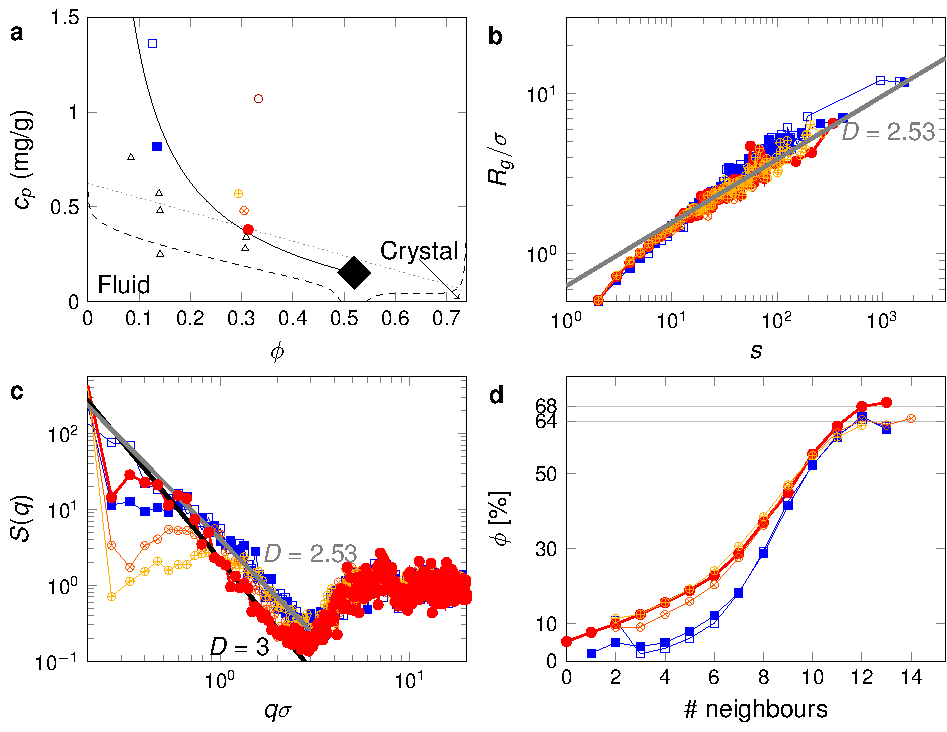
\includegraphics{phase_separation.pdf}
 \caption{{\bf Different routes of viscoelastic phase separation.} 
{\bf a,} Phase diagram. Gray areas are equilibrium fluid and crystal regions. The dashed and continuous lines are the metastable gas-liquid binodal and spinodal respectively. The black diamond marks the critical point. Empty black triangles are experimental point showing a fluid behaviour. The other symbols are the experimental points showing gel behaviour, consistently used in all panels. The dotted lines are the gas-liquid tie lines determined experimentally, with arrow heads indicating measured gas and liquid compositions.
{\bf b,} Radius of gyration ($R_g$) as a function of cluster size ($s$) for all state points at percolation. The
 gray line represents the fractal dimension of the random gelation universality class.
{\bf c,} Structure factors for the late stages of the gelation process. The gray and black lines represents respectively random gelation and compact fractal dimensions.
{\bf d,} Local volume fraction around a colloidal particle, as a function of the number of nearest neighbours of the particle for the state points in the very late stage. Horizontal lines stress the value at 12 neighbours.
 }
 \label{fig:phase_separation}
\end{figure*}



\clearpage

\begin{figure*}[!t]
 \centering
 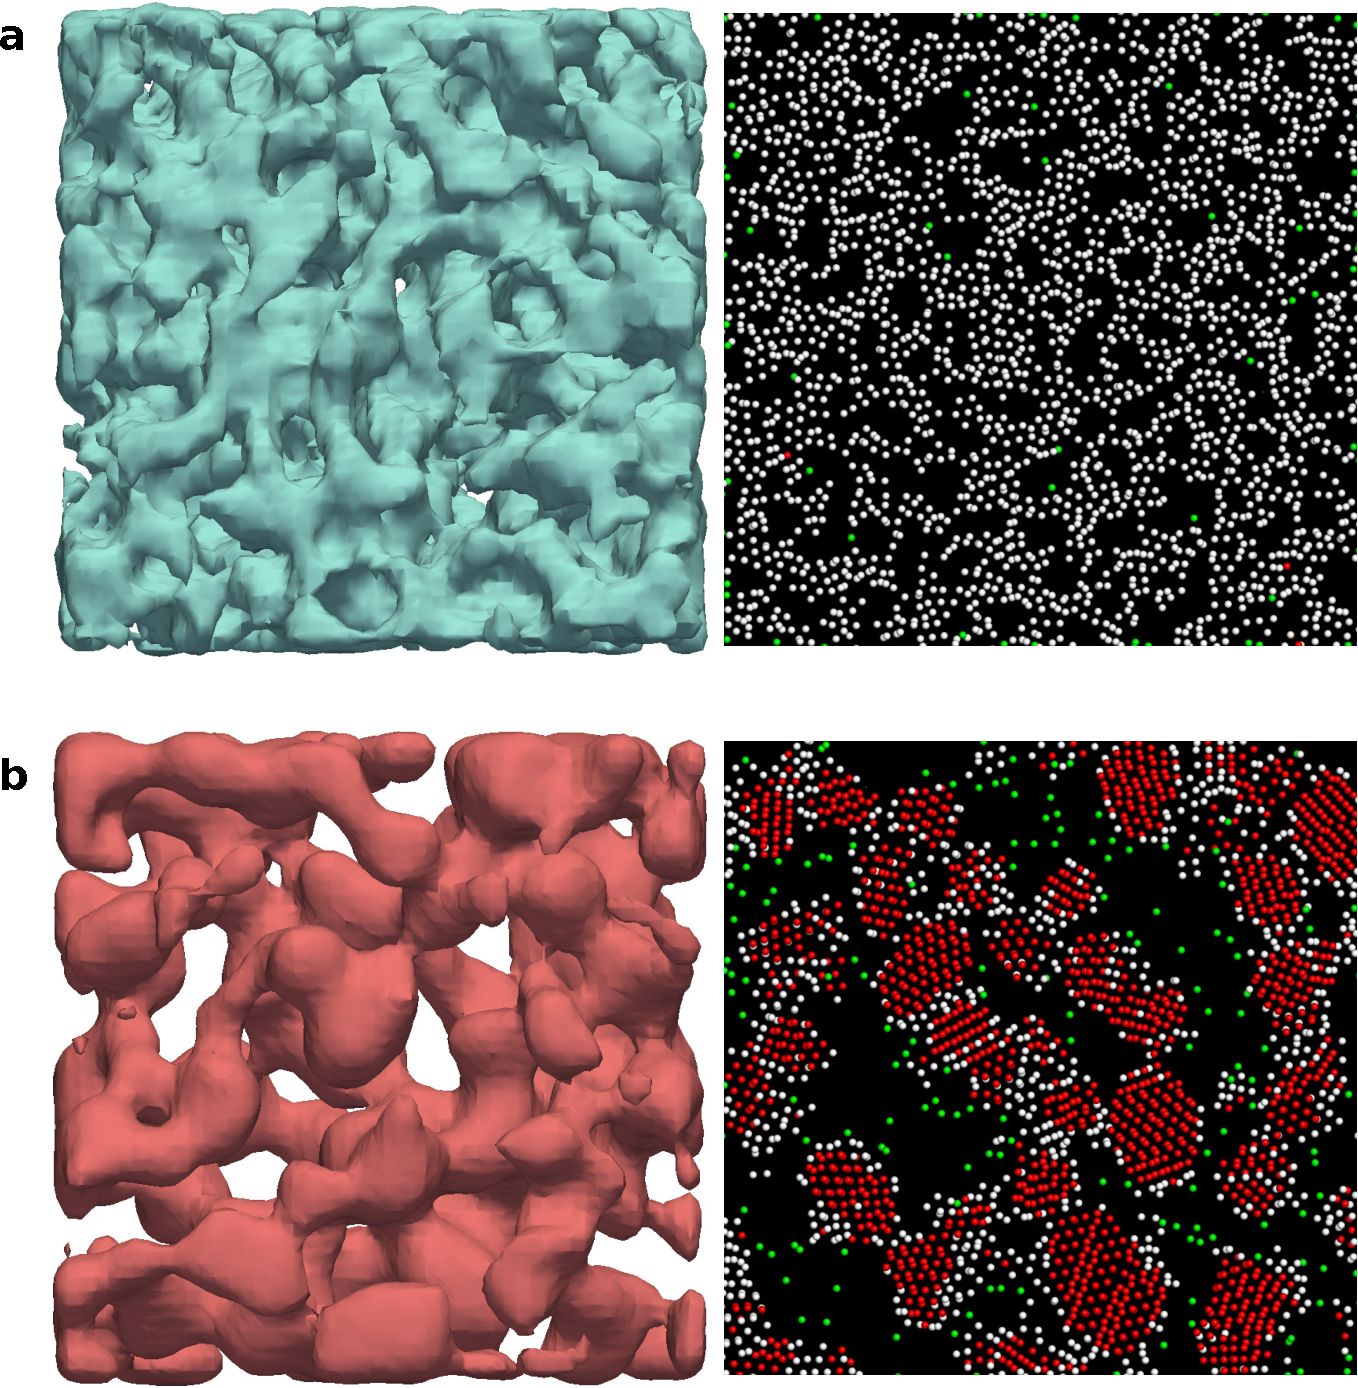
\includegraphics[width=12cm]{fig2}
 % crystal_size.eps: 0x0 pixel, 300dpi, 0.00x0.00 cm, bb=(atend)
\caption{\textcolor{red}{{\bf Percolated network structures.} {\bf a:} gel; {\bf b:} crystal-gel. The gel state is obtained from the state
point $\phi\approx 0.30$ and $c_p=1.07$ mg/g, while the crystal-gel is obtained at the same $\phi$ but
at lower polymer concentration, $c_p=0.38$ mg/g. On the left, the network is represented as a continuous field that has
been obtained by applying a gaussian filter to the position of the particles (of width equal to the inter-particle distance) and
plotting the surface which bounds the highest 20 \% values of the field. We can clearly see not only the percolated nature of both networks, 
but also the difference in the smoothness of the network surface between amorphous and crystal gels. 
On the right, slabs of 5 particle diameter thickness are plotted,
with particles coloured with the same colour scheme as in Fig.~\ref{fig:transitions}: red (crystal), green (gas particles), white (liquid particles). 
We note that very few liquid particles remain and the network is almost crystalline.}} 
\label{fig:network}
\end{figure*}

\clearpage

\begin{figure}[!t]
 \centering
 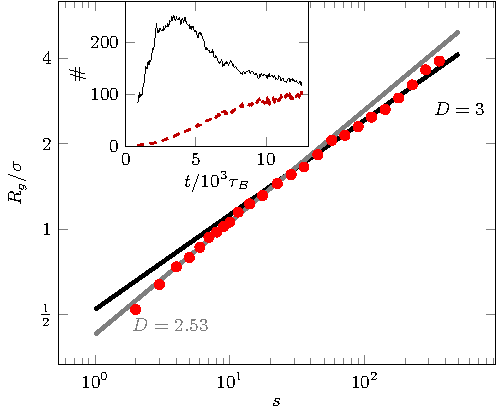
\includegraphics{characterisation}
 % crystal_size.eps: 0x0 pixel, 300dpi, 0.00x0.00 cm, bb=(atend)
\caption{{\bf Characterization of the crystal-gel.} {\bf a,} Time evolution of the average size of the crystals (blue line) and the number of crystals (red line) for the state point $\phi\approx 0.30$ and $c_p=0.38$ mg/g. {\bf b,} Radius of gyration of crystalline nuclei at the late stages of gelation for the same state point.} 
 \label{fig:crystals}
\end{figure}

\clearpage 

\begin{figure*}[!t]
 \centering
 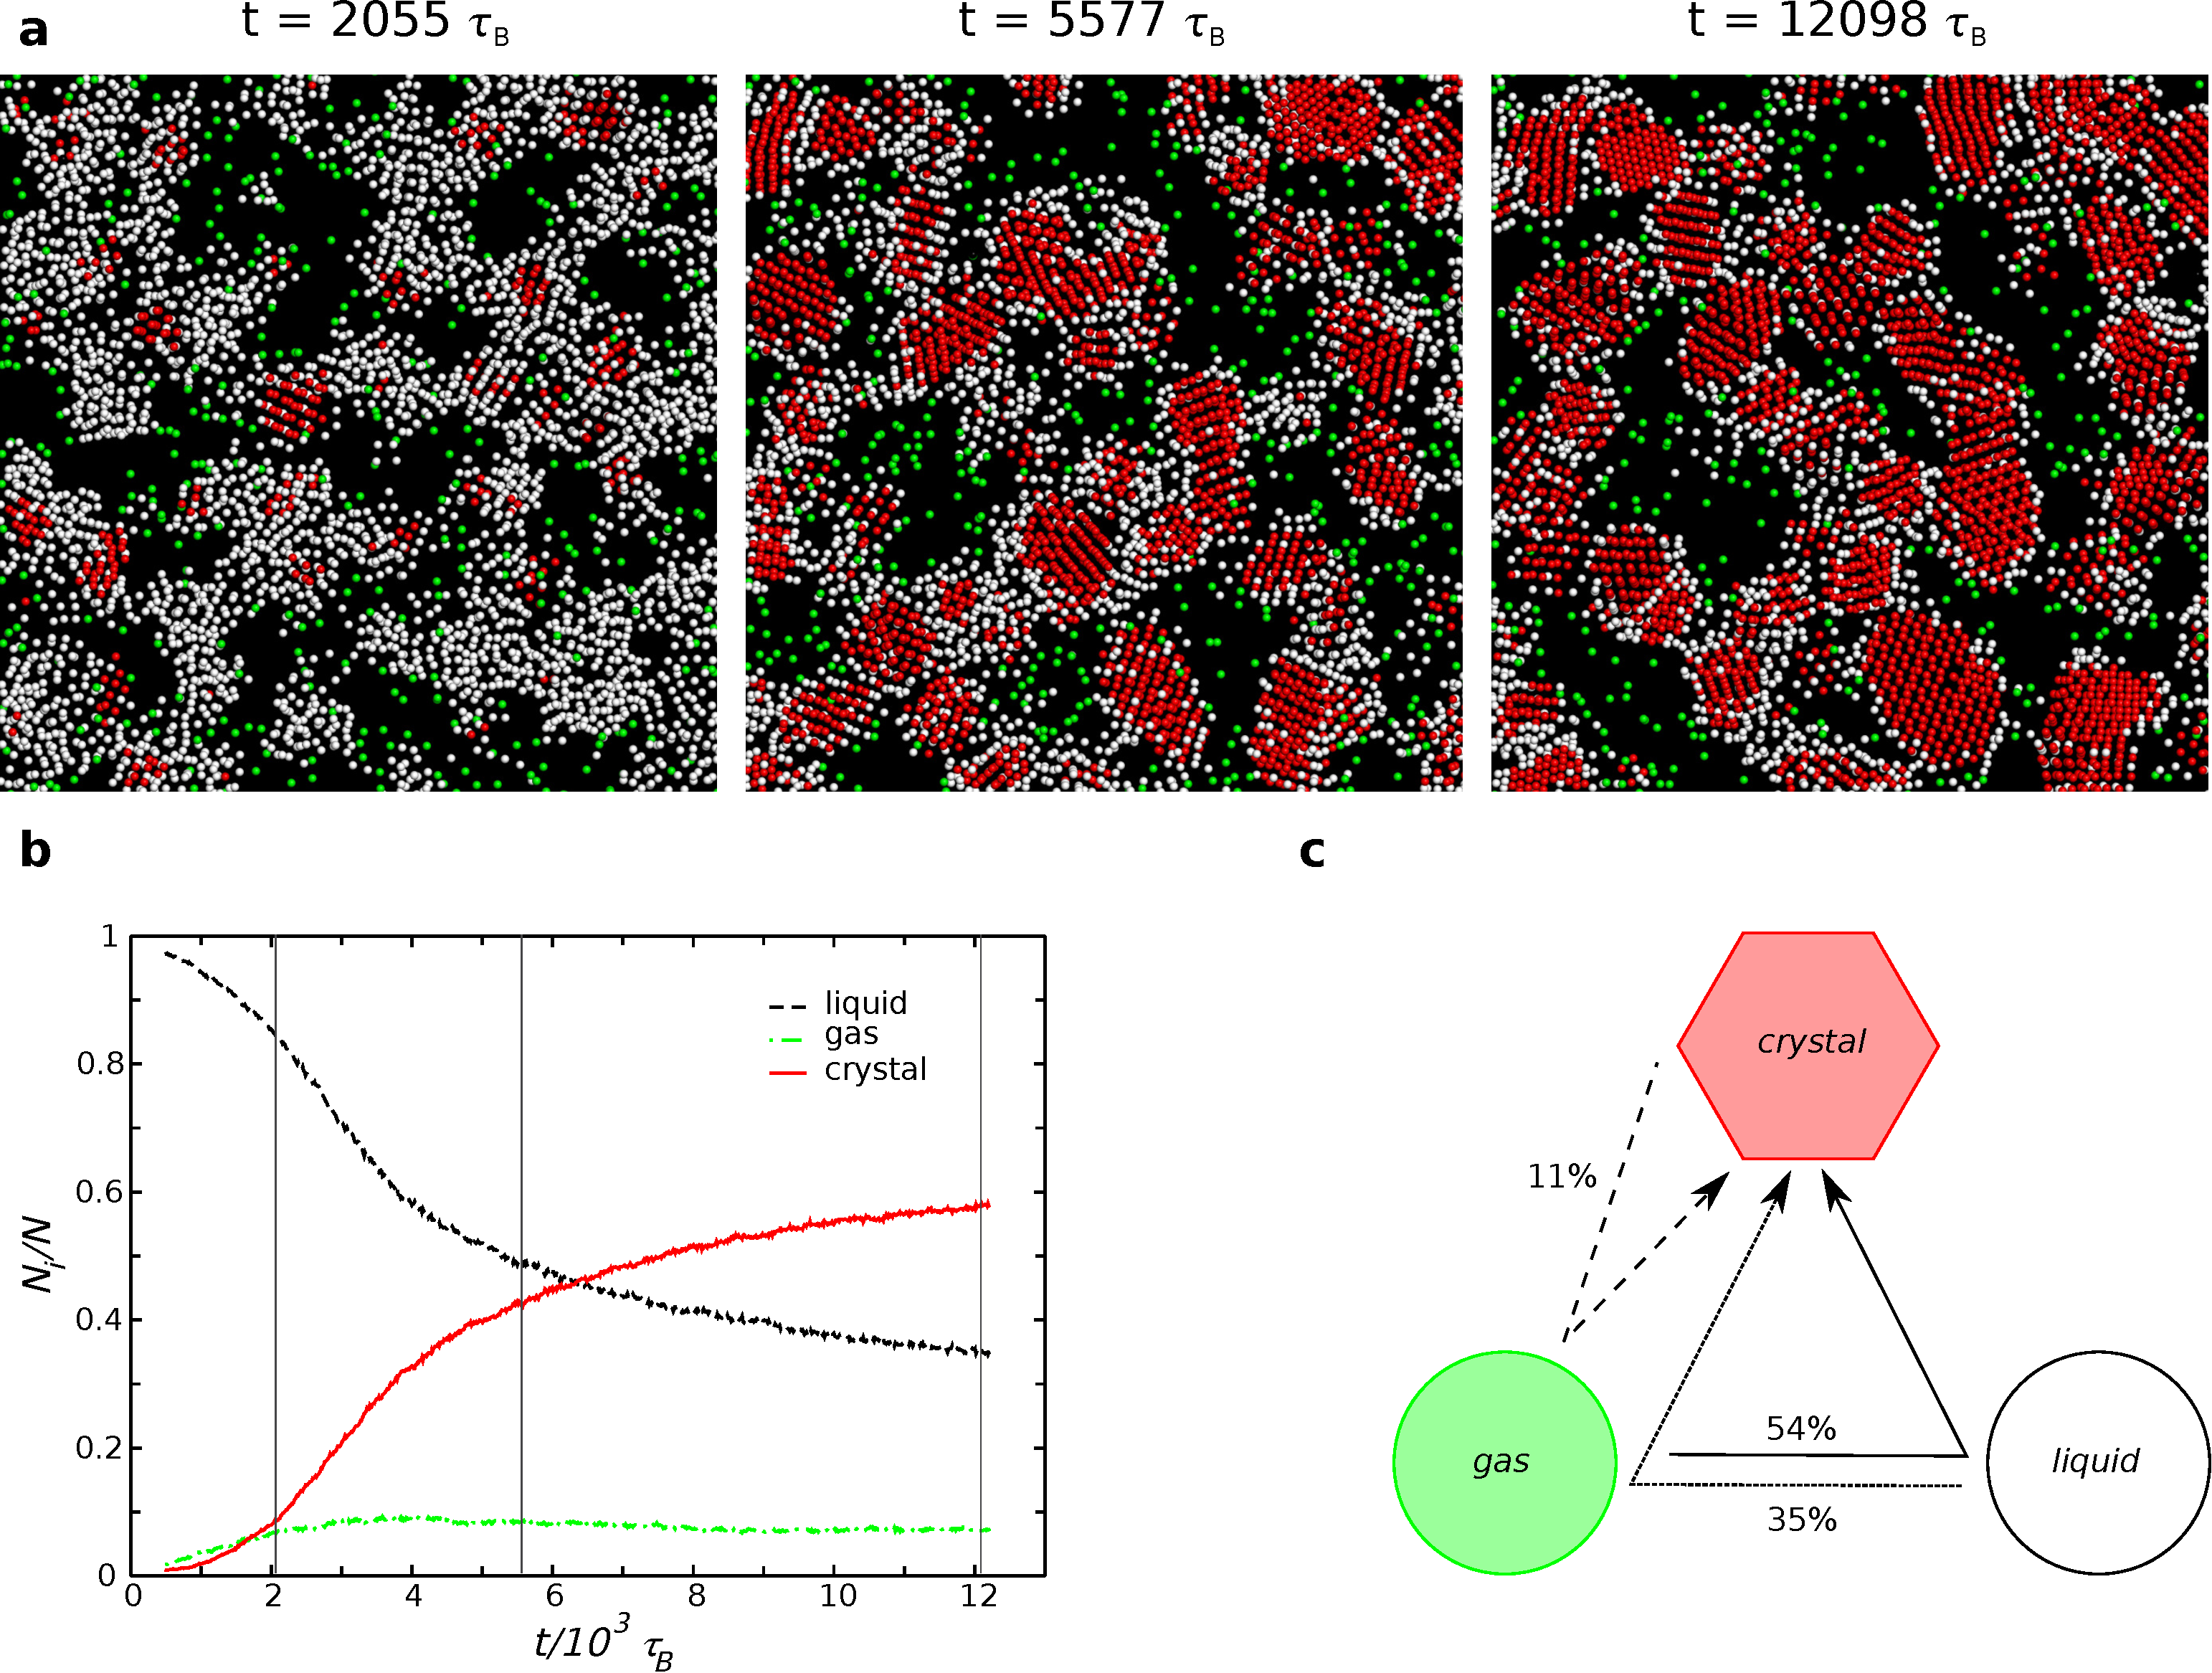
\includegraphics[width=14cm]{fig4}
 % snapshots.eps: 0x0 pixel, 300dpi, 0.00x0.00 cm, bb=0 -1 2256 735
 \caption{\textcolor{red}{{\bf Crystal gel formation.}  
{\bf a,} Reconstructions from confocal coordinates at $\phi\approx 0.30$ and $c_p=0.38$ mg/g. Depth of view is $5\sigma$. Particles are drawn to scale and coloured according to their phase. Red: crystal; white: liquid; green: gas. 
{\bf b,} Fraction of particles for each phase. Gray vertical lines indicate the times shown in panel a. 
{\bf c,} Each particle during its trajectory changes between three states: gas, liquid and crystal. Direct crystallization accounts for 54\% of particles trajectories in which
gas or liquid particles transition to the crystal state without liquid evaporation or crystal de-sublimation. The Bergeron process accounts for 35\% of particle trajectories in which liquid particles
transition to the gas state before crystallizing. Ostwald ripening accounts for 11\% of particle trajectories in which crystal particle transition to the gas state before returning
to the crystal state.}}
\label{fig:transitions}
\end{figure*}

\end{document}



